\documentclass[12pt,a4paper]{article}
\usepackage{fontspec}
\setmainfont{Times New Roman}
\usepackage[a4paper,left=26mm,right=26mm,top=28mm,bottom=26mm,headheight=16pt]{geometry}
\usepackage{fancyhdr}
\usepackage{lastpage}
\usepackage{amsmath}
\usepackage{graphicx}
\usepackage{booktabs}
\usepackage{caption}
\captionsetup[table]{position=top}
\captionsetup[figure]{position=bottom}
\usepackage[hidelinks]{hyperref}

\newcommand{\ProblemLetter}{B}
\newcommand{\TeamNumber}{SWBMCM2613050}
\newcommand{\PaperTitle}{Rapid UAV Localization via Coordinated Mobile Vehicles}
\newcommand{\TeamPageHeader}{%
  \fancyhf{}%
  \fancyhead[L]{Team\#\TeamNumber}%
  \fancyhead[R]{Page \thepage\ of \pageref*{LastPage}}%
  \renewcommand{\headrulewidth}{0.4pt}%
}
\fancypagestyle{fancy}{\TeamPageHeader}
\fancypagestyle{plain}{\TeamPageHeader}
\renewcommand{\contentsname}{Content}
\setcounter{tocdepth}{1}
\graphicspath{{../figures/}}

\begin{document}
\pagestyle{fancy}
\thispagestyle{empty}
\begin{center}
\begin{tabular}{@{}lll@{}}
  Problem Chosen & 2026 ShuWei Cup & Team Control Number \\
  \ProblemLetter & Summary Sheet & \TeamNumber
\end{tabular}

\vspace{1em}
{\Large\bfseries\PaperTitle}
\end{center}
\section*{Summary}
An observation and dispatch prototype was evaluated on the Problem B field. The shortest feasible horizontal observation range for T1 is 7.582 m. For T2, the selected stations give a first-order horizontal RMS error of 0.1436 m. The beam-search schedule starts its last observation at 11.03 s compared with 11.72 s under the nearest-arrival rule. The pointing error allowance is met up to about 66.8 m of travel. Across 28 selected disturbance cases, replanning improves 23, ties 4, and worsens 1 by the prescribed ranking.

\noindent\textbf{Keywords:} Bearing-only localization; vehicle scheduling; uncertainty; rescheduling

\clearpage
\tableofcontents
\clearpage

\section{Observation Region and Station Selection}

Position is measured east and north from the southwest corner. A station is admissible when a vehicle disc fits within the field without entering a building, its finite camera-to-target segment misses every closed building prism, and the target elevation is within the gimbal limits. A slab intersection retains contact at a single parameter value, which makes tangency occluding [1].

With the target above the camera, the upper elevation limit implies that the horizontal distance is at least the height difference divided by the tangent of the upper limit. A feasible point on that inner circle therefore attains the upper bound on inverse-range quality. A one-degree angular sweep identifies a reproducible representative among the tied sampled stations.

The selected station is (77.516, 72.593) m. Its elevation is 80.0 degrees and its inverse-range quality is 0.13189 per metre. The plotted region is a one-metre raster, while the selected station uses continuous coordinates.

\[r \ge (H-h)/\tan\beta_{\max},\qquad Q=1/r\]

\begin{figure}[htbp]

\centering

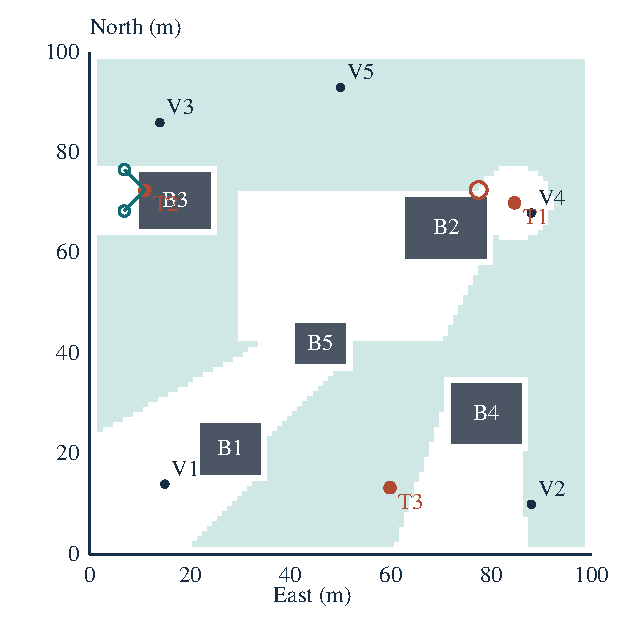
\includegraphics[width=0.8\linewidth]{b_geometry}

\caption{Observable footprint for T1 (light teal), a selected station (red ring), and T2 viewing rays (teal).}

\end{figure}

\section{Dual-Station Localization for T2}

Let r1 and r2 be the horizontal sensor ranges, and let gamma be the smaller angle between the two bearings. The first-order error normal to each bearing is range times the angular error in radians. The two normal equations determine the horizontal displacement. Inverting their two-by-two coefficient matrix, then taking the trace of the propagated covariance, gives sigma squared times (r1 squared plus r2 squared) divided by sin squared gamma [2].

The RMS metric is the square root of that trace. Baseline, ranges, and crossing angle obey the cosine rule. The metric diverges near parallel or antiparallel bearings. An observation boundary is a separate issue because a small station shift can invalidate visibility or travel.

Vehicles V3 and V5 are assigned to (6.914, 68.385) m and (6.914, 76.615) m. Their travel times are 6.46 s and 15.37 s. The baseline is 8.229 m, and the crossing angle is 90.0 degrees.

Both ranges meet the pitch-imposed lower bound and the sine factor attains one. The chosen feasible pair attains the lower bound for the specified first-order RMS criterion. This claim applies to the local metric and the nominal target position.

\[\operatorname{RMS}\approx\frac{\sigma_\theta\sqrt{r_1^2+r_2^2}}{|\sin\gamma|}\]

\section{Multi-Alert Vehicle Scheduling}

Shortest routes on a waypoint graph use conservative rectangular expansions of the buildings by the disc radius. Expanded corners with a small clearance and the start and finish points form the graph. This makes each computed route feasible for the vehicle disc, while potentially excluding shorter rounded-corner paths [3].

Each task selects two different vehicles and two distinct, nondegenerate stations. Driving, slewing, waiting for the partner, simultaneous observation, and reset occupy each vehicle in that order. The two gimbal axes can move together. Availability for the next drive is the end of the current task's reset.

The search enumerates alert orders and retains a bounded beam of partial schedules per order. The best feasible schedule across two search budgets is carried forward to the disturbance study. The baseline visits alerts in input order and selects the pair minimizing the later driving arrival, using the same route, visibility, geometry and synchronization tests.

The last start is 11.03 s for beam search and 11.72 s for nearest assignment, a difference of 0.69 s. The comparison is between evaluated feasible schedules. No global optimality claim is made.

\[t_{\mathrm{start},j}=\max_{i\in A_j}t_{\mathrm{ready},i,j},\qquad\min\max_j t_{\mathrm{start},j}\]

\begin{figure}[htbp]

\centering

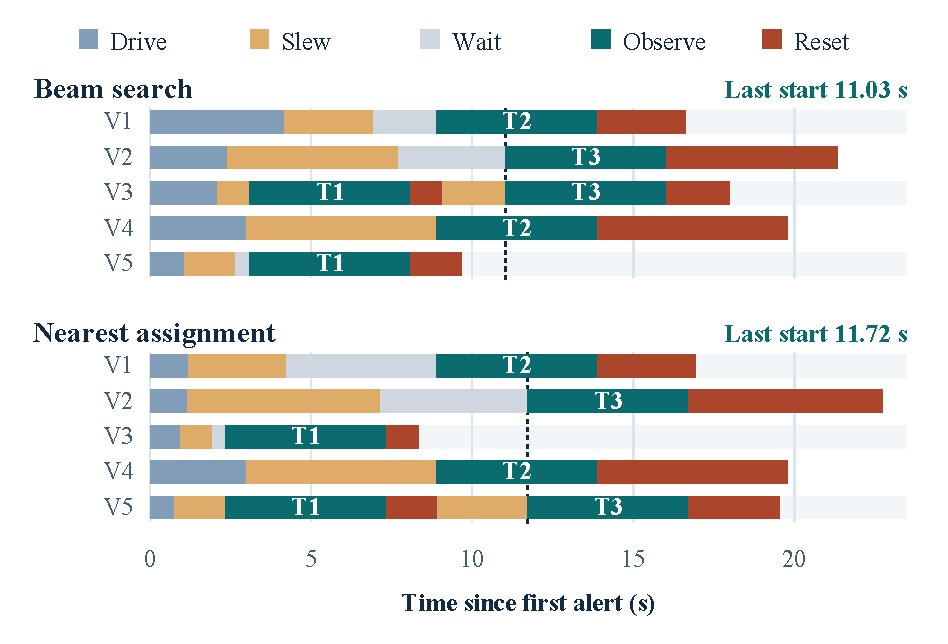
\includegraphics[width=0.8\linewidth]{b_timeline}

\caption{Per-vehicle timeline for beam search (B) and nearest assignment (N).}

\end{figure}

\section{Horizontal Pointing Error}

By rotational symmetry, put the target on the positive horizontal axis. The position error changes the bearing through atan2 of the lateral displacement and the perturbed longitudinal range. Here X and Y are the position-estimate errors along and across the nominal bearing. The two independent gimbal errors add as a normal variable. Their convolution with the position-induced angle is integrated over wrapped intervals about zero.

Composite Simpson integration is applied to the standardized position variables. A normal CDF integrates the gimbal component conditional on those variables. A bisection search finds the relevant coverage crossing. An independent first-order approximation propagates the lateral position variance divided by squared range, plus the two gimbal variances [4].

The nonlinear threshold is 66.837 m; the coarser integration gives 66.837 m and the linearized estimate gives 66.922 m. At 80 m, the admissible nonnegative parameters satisfy a + 80 b no greater than approximately 1.6367 m.

The linearized variance shares near the threshold are 84.6\% for the vehicle position, 9.9\% for gimbal offset, and 5.5\% for gimbal control.

\[\Delta\psi=\operatorname{wrap}\left(\operatorname{atan2}(-Y,r-X)+\epsilon_0+\epsilon_c\right)\]

\begin{figure}[htbp]

\centering

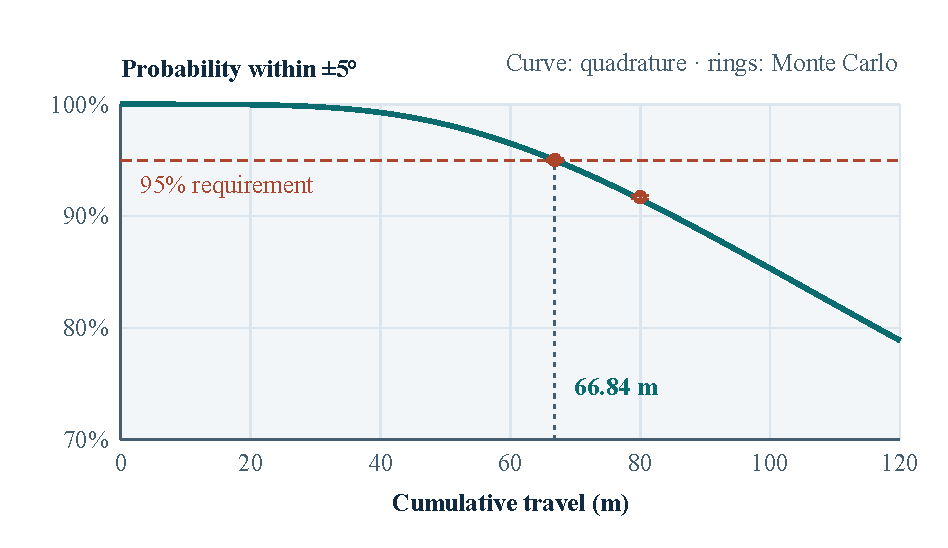
\includegraphics[width=0.8\linewidth]{b_coverage}

\caption{Calculated probability of remaining within the two-sided pointing limit.}

\end{figure}

\section{Rescheduling After Disturbances}

At time zero both policies begin with the same nominal plan. In the fixed plan, a new alert remains unassigned and a scheduled observation involving a failed vehicle cannot start after failure. The surviving vehicles otherwise retain their nominal instructions. A replan first recovers positions by interpolation along the issued routes, carries forward valid observations already started, and removes the failed vehicle [5].

During communication loss, the nominal instructions continue. Reassignment is available only at recovery. Surviving vehicles in interrupted pre-observation phases reset conservatively before accepting new movement. The plan ranks the number of valid observations started by the deadline first and the last observation start second.

The main outage interpretation uses an absolute recovery time. The longest duration in the accompanying prose is tested separately as a sensitivity case. Failure identities are enumerated. New-alert locations are representative discrete cases, and the resulting counts are not population probabilities.

Replanning improves 23 cases, ties 4, and worsens 1. In failure\_V5, the fixed plan gives a completion ratio of 1.00 and a latest start of 11.03 s. Replanning gives 1.00 and 12.93 s. Canceling a viable assignment can waste prior positioning.

\[\operatorname{lex\,max}\;(\eta,-t_{\rm last}),\qquad\eta=k/N\]

\begin{figure}[htbp]

\centering

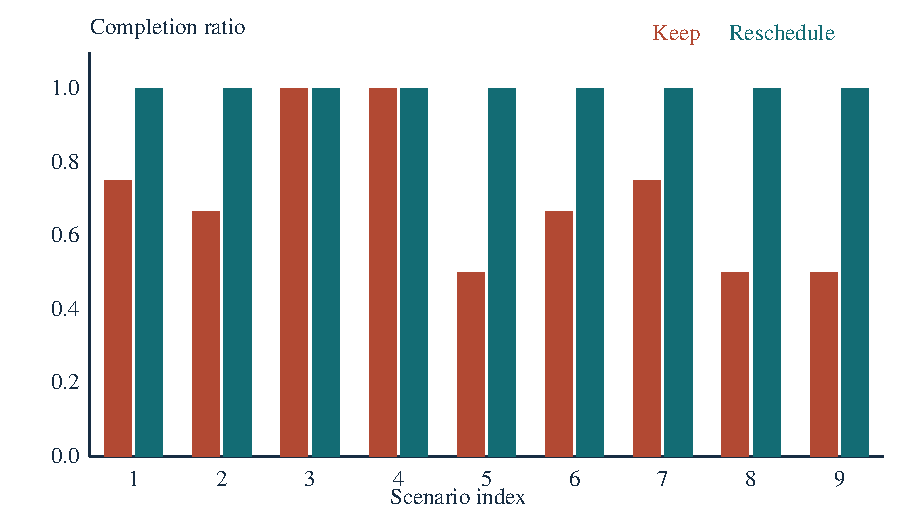
\includegraphics[width=0.8\linewidth]{b_disturbances}

\caption{Completion ratios across selected cases, in order: new\_1, failure\_V1, failure\_V5, outage\_upper\_time, new\_failure\_V1, failure\_outage\_V1, new\_outage, all\_V1, all\_duration\_sensitivity.}

\end{figure}

\section{Paired Scenario Results}

For each row, the completion fraction counts alert starts within the evaluation window. The last-start column follows the specified horizon convention when an alert is unfinished.

\begin{table}[htbp]

\centering

\caption{Completion ratios and latest-start times in seconds}

\begin{tabular}{@{}lrrrr@{}}

\toprule

Scenario & Keep ratio & Keep time & Replan ratio & Replan time \\

\midrule

new 1 & 0.75 & 60.00 & 1.00 & 18.32 \\

new 2 & 0.75 & 60.00 & 1.00 & 19.44 \\

new 3 & 0.75 & 60.00 & 1.00 & 20.26 \\

failure V1 & 0.67 & 60.00 & 1.00 & 13.40 \\

failure V2 & 0.67 & 60.00 & 1.00 & 13.40 \\

failure V3 & 0.67 & 60.00 & 1.00 & 13.40 \\

failure V4 & 0.67 & 60.00 & 1.00 & 13.40 \\

failure V5 & 1.00 & 11.03 & 1.00 & 12.93 \\

outage interior & 1.00 & 11.03 & 1.00 & 11.03 \\

outage upper time & 1.00 & 11.03 & 1.00 & 11.03 \\

outage upper duration & 1.00 & 11.03 & 1.00 & 11.03 \\

new failure V1 & 0.50 & 60.00 & 1.00 & 24.51 \\

failure outage V1 & 0.67 & 60.00 & 1.00 & 35.91 \\

all V1 & 0.50 & 60.00 & 1.00 & 36.15 \\

new failure V2 & 0.50 & 60.00 & 1.00 & 20.57 \\

failure outage V2 & 0.67 & 60.00 & 1.00 & 33.73 \\

all V2 & 0.50 & 60.00 & 1.00 & 34.83 \\

new failure V3 & 0.50 & 60.00 & 1.00 & 25.23 \\

failure outage V3 & 0.67 & 60.00 & 1.00 & 34.12 \\

all V3 & 0.50 & 60.00 & 1.00 & 36.46 \\

new failure V4 & 0.50 & 60.00 & 1.00 & 21.09 \\

failure outage V4 & 0.67 & 60.00 & 1.00 & 33.10 \\

all V4 & 0.50 & 60.00 & 1.00 & 36.15 \\

new failure V5 & 0.75 & 60.00 & 1.00 & 20.57 \\

failure outage V5 & 1.00 & 11.03 & 1.00 & 11.03 \\

all V5 & 0.75 & 60.00 & 1.00 & 32.00 \\

new outage & 0.75 & 60.00 & 1.00 & 32.00 \\

all duration sensitivity & 0.50 & 60.00 & 1.00 & 39.83 \\

\bottomrule

\end{tabular}

\end{table}

\section{Validation, Limitations, and References}

The implementation checks station visibility, collision-free route segments, joint observation start, task duration, and nonoverlapping vehicle timelines. Replans are checked against the recovery time and failed vehicle identity. The search is deterministic. Auditable numerical outputs and the full scenario timelines are stored separately. A separate seeded Monte Carlo check evaluates exact bearing intersections and the wrapped pointing error. A wider beam can perform worse under partial-plan pruning, so the best previously found feasible schedule is retained.

Across 100,000 draws, the exact-intersection RMS was 0.1439 m. Pointing coverage was 0.95016 at the threshold (Wilson interval 0.94879 to 0.95149) and 0.91688 at the specified 80 m check distance.

The model treats targets as stationary, ignores interactions between moving vehicles as in the nominal timing assumptions, and uses finite station candidates. The scenario study is conditional on the stated continuation and cancellation rules. Further sensitivity checks should examine station discretization, clearance, the chosen outage interpretation, and sample coverage.

[1] Liang and Barsky. A New Concept and Method for Line Clipping. ACM Transactions on Graphics, 1984. doi:10.1145/357332.357333.

[2] Bishop et al. Optimality Analysis of Sensor-Target Localization Geometries. Automatica, 2010. doi:10.1016/j.automatica.2009.12.003.

[3] Dijkstra. A Note on Two Problems in Connexion with Graphs. Numerische Mathematik, 1959. doi:10.1007/BF01386390.

[4] JCGM. Guide to the Expression of Uncertainty in Measurement, Section 5, 2008. doi:10.59161/JCGM100-2008E.

[5] Pillac et al. A Review of Dynamic Vehicle Routing Problems. European Journal of Operational Research, 2013. doi:10.1016/j.ejor.2012.08.015.

[6] OpenAI ChatGPT (Codex, GPT-6 series), used on 20 November 2026.

\section{AI Tool Usage Report}

Tool: OpenAI ChatGPT (Codex, GPT-6 series). Date of use: 20 November 2026.

Prompt summary: use the supplied Problem B statement and transcribed parameters to develop and evaluate an end-to-end prototype and produce a reproducible English draft.

Output and adoption in this draft: AI assistance was used for source transcription, model and solver design, coding and validation, chart generation, interpretation, and drafting. These contributions cover all sections and the associated code and figures [6].

Human revision status: this version records the AI-produced draft. Subsequent human verification, edits, or replacement analyses should be recorded in the AI-use log.

\end{document}
